\documentclass[journal]{IEEEtran}

%\usepackage[pass,letterpaper]{geometry}              %This package needs to be enaled when dvi--->ps----->PDF
\usepackage{stmaryrd, amsfonts, mathptmx, mathtools, array, siunitx, subfigure, graphicx,balance }
\graphicspath{{./fig/}}
\usepackage{multirow, indentfirst, cite, verbatim, keyval, textcomp, enumerate, calc, microtype, hyperref, makecell, booktabs, tabularx}



\usepackage[colorlinks,linktocpage]{hyperref}
\hypersetup{
   colorlinks   = true,                               %Colours links instead of ugly boxes
   urlcolor     = blue,                               %Colour for external hyperlinks
   linkcolor    = blue,                               %Colour of internal links
   citecolor    = red,                                %Colour of citations
   setpagesize  = false,
   linktocpage  = true,
}

\IEEEoverridecommandlockouts

\begin{document}
\raggedbottom

\title{\ \\ \LARGE\bf Smart School Food Service Analysis: AI-Driven Demand Forecasting and Waste Reduction Using Fairfax County Public Schools Data}

\author{
\IEEEauthorblockN{
Jupiter Kang\IEEEauthorrefmark{1},
Crystal Kao\IEEEauthorrefmark{1},
Alonso Romero\IEEEauthorrefmark{1},
Amir Jafari\IEEEauthorrefmark{2}
}

\IEEEauthorblockA{
\IEEEauthorrefmark{1}Graduate Students, M.S. in Data Science, The George Washington University, Washington, D.C.\\
Emails: jk720@gwu.edu, crystal.kao@gwu.edu, alonso.romero@gwu.edu
}

\IEEEauthorblockA{
\IEEEauthorrefmark{2}Assistant Professor, Data Science Program, The George Washington University, Washington, D.C.\\
Email: ajafari@gwu.edu
}
}

\maketitle

%*********************************************************************************************************************************************************************************************************************
\begin{abstract}
Food waste in U.S. public schools is a major economic and environmental problem, with about 530,000 tons of food discarded each year and \$1.7 billion in losses \cite{wwl}. Fairfax County Public Schools (FCPS) in Virginia plans to solve this problem by using data to reduce waste and improve efficiency. While digital data from Point-of-Sale (POS) systems and kitchen records is widely available, most districts, including FCPS, lack the tools to transform this data into actionable insights. This study analyzes FCPS data from May 2025 to pinpoint inefficiencies, identify high- and low-demand items, and reveal patterns by region and school level. Our main goal is to provide clear, practical recommendations that allow FCPS to serve meals more sustainably and efficiently.
\end{abstract}
%*********************************************************************************************************************************************************************************************************************
\section{INTRODUCTION}

School cafeterias struggle to serve healthy meals while reducing waste. As schools become more diverse, relying on old ways of managing and determining how much food to produce only worsens the problem, emphasizing the need for data-driven solutions. Although digital data from POS systems and kitchen records is available, most school districts lack analytics tools to integrate and analyze it. Fairfax County Public Schools (FCPS) provided us with production data from May 2025 to support a solution to this challenge.

%*********************************************************************************************************************************************************************************************************************
\section{RELATED WORK}

\subsection{The Cafeteria as a Classroom}

In addition to data-driven solutions, some schools around the country have implemented behavioral interventions worth considering for FCPS. In one example, Bridget Huber describes a study at Lovin Elementary School in Lawrenceville, Georgia, conducted during "Taco Day" \cite{huber}. Gerin Hennebaul and a group of students sorted leftover milk, fruit, vegetables, and other foods into buckets. They found that 600 pounds of food were wasted, including 75 pounds of fruit and vegetables and 120 pounds of uneaten food \cite{huber}. This magnitude of food waste being transported to landfills causes a concern of methane emissions rising, ultimately harming the environment. To address this, Lovin Elementary told students that milk at lunch was optional, set up a shared table for uneaten food for everyone to share with each other, and increased composting efforts \cite{huber}.

\subsection{Study of Waste Production at a Private School}

Building on these approaches, other research teams also studied which foods were most wasted to better target solutions. In \cite{mulhollem}, a study by Christine Costello, assistant professor at Penn State, focused on a private school in Columbia, Missouri. The school was chosen because its administrators wanted to improve cafeteria sustainability, and it includes an unusual mix of students from ages four to eighteen \cite{mulhollem}. The main finding is that the study assessed the environmental and cost impacts of food served and wasted in the cafeteria, including how much was served, consumed, and discarded, as well as the nutritional value lost \cite{mulhollem}.
%*********************************************************************************************************************************************************************************************************************

\section{INTEGER LINEAR PROGRAMMING OPTIMIZATION}

Integer linear programming (ILP) optimizes problems with integer variables, which is essential for FCPS since school meals are ordered in whole units. Our goal is to minimize costs, reduce waste, maximize savings, and provide cafeteria managers with precise, data-driven recommendations.

\subsection{Optimization Model Formulation}
We created an ILP model to help FCPS cafeteria managers reduce food waste by selecting the optimal number of menu items. The model aims to reduce total costs by balancing production expenses with a waste penalty that aligns with FCPS needs.

\

\subsubsection{Decision Variables}
Let $x_j$ be the integer quantity of menu item $j$ to be produced.

\

\subsubsection{Parameters}
\begin{itemize}
    \item $c_j$: The unit production cost for item $j$.
    \item $w_j$: The waste penalty associated with item $j$ (derived from historical leftover rates).
    \item $d_j$: The predicted demand for item $j$.
\end{itemize}

\

\subsubsection{Objective Function}
The objective is to minimize the Total Cost ($C_T$), balancing the financial cost of meals and the environmental cost of waste. Based on our "Minimized Cost" metric, the objective function is:

\begin{equation}
    \text{Minimize } Z = \sum_{j=1}^{n} (c_j + \lambda w_j) x_j
\end{equation}
where $\lambda$ represents the waste penalty weight (set to 0.1 in our analysis).

\

\subsubsection{Constraints}
To align production with student needs and minimize waste, we used a production bounds constraint. This constraint keeps production within a defined range. The range is based on estimated demand:

\begin{equation}
    L_{s,j} \leq x_{s,j} \leq U_{s,j} \quad \forall s, \forall j
    \label{eq:bounds}
\end{equation}

\begin{table}[t]
    \caption{Production Bounds Based on School Size}
    \label{tab:production_bounds}
    \centering
    \begin{tabular}{cc}
        \toprule
        \textbf{Student Population} & \textbf{Production Bounds $(L, U)$} \\
        \midrule
        0--499 & (0.80, 1.20) \\
        500--999 & (0.85, 1.15) \\
        1000--1499 & (0.90, 1.10) \\
        1500--1999 & (0.95, 1.05) \\
        2000--2499 & (0.96, 1.04) \\
        2500--2999 & (0.97, 1.03) \\
        3000--3499 & (0.98, 1.02) \\
        3500+ & (0.99, 1.01) \\
        \bottomrule
    \end{tabular}
\end{table}

In our optimization model, we scale the bounds by size multipliers tied to each school's student population (\autoref{tab:production_bounds}). We see that smaller schools have a longer range than the larger schools. Schools with smaller populations are more volatile as a small change in daily events can result in a massive waste percentage impact. For example, a school of 500 students one day has a flu outbreak and 50 students call in sick, that is a 10\% reduction in demand for that day. A wider buffer takes account for this unpredictability. On the other hand, a school of 3000 students that has 50 students call out one day would result in a 1.6\% reduction in demand. The buffer would tighter as attendance is more stable. This is represented by:

\begin{equation}
    \begin{aligned}
        L_{s,j} &= \alpha_s \cdot d_{s,j} \\
        U_{s,j} &= \beta_s \cdot d_{s,j}
    \end{aligned}
\end{equation}

Where coefficients $(\alpha_s, \beta_s)$ are determined by school size:

\[
(\alpha_s, \beta_s) = 
\begin{cases} 
    (0.80, 1.20) & \text{if } s \in \text{0-499} \\
    (0.85, 1.15) & \text{if } s \in \text{500-999} \\
    (0.90, 1.10) & \text{if } s \in \text{1000-1499} \\
    (0.95, 1.05) & \text{if } s \in \text{1500-1999} \\
    (0.96, 1.04) & \text{if } s \in \text{2000-2499} \\
    (0.97, 1.03) & \text{if } s \in \text{2500-2999} \\
    (0.98, 1.02) & \text{if } s \in \text{3000-3499} \\
    (0.99, 1.01) & \text{if } s \in \text{3500+}
\end{cases}
\]

Here, $d_{s,j}$ represents the demand for item $j$ at school $s$. In addition to these production bounds, we require that the production quantities, represented by the decision variables, be non-negative integers, enforced by:

\begin{equation}
    x_{s,j} \in \mathbb{Z}^+ \quad \forall s, \forall j
\end{equation}

Finally, we included two budget constraints in the model: a per-school budget constraint ($B_s$), and a system-wide total budget constraint ($B_{total}$):

\begin{equation}
    \sum_{j} (c_{j} \cdot  x_{s,j}) \leq B_{s}
    \label{eq:school_budget}
\end{equation}

\begin{itemize}
    \item $c_j$: The unit production cost for item $j$.
    \item $x_{s,j}$: Quantity of items produced by school $s$.
    \item $B_s$: The maximum budget allocated to school $s$.
\end{itemize}

The per-school budget constraint ensures equity across all the schools in the system. It prevents larger schools from "hoarding" the budget, allowing every school to have enough funds to meet its specific demand.

\begin{equation}
    \sum_{s}\sum_{j} (c_{j} \cdot x_{s,j}) \leq B_{total}
    \label{eq:total_budget}
\end{equation}

The system-wide budget constraint ensures sustainability. It ensures that the spending across the county does not exceed the allocated \$139,144,760 budget \cite{fcpsbudget}.

%*********************************************************************************************************************************************************************************************************************
\section{RESULTS}

\subsection{Financial Impact Analysis}

\begin{figure}[t]
    \centering
    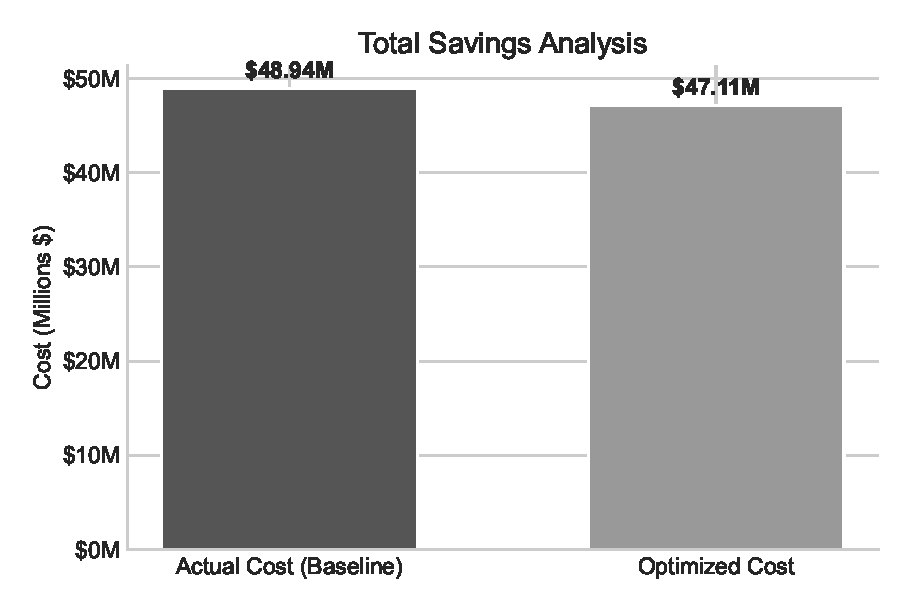
\includegraphics[width=\linewidth]{fig/total_savings_bar_bw.eps}
    \caption{Overall Savings Analysis. This comparison shows the financial impact of the optimization model across the system. The dark gray bar shows the estimated actual annual baseline cost (\$48.94M), and the light gray bar shows the lower cost reached with the optimized menu planning model (\$47.11M).}
    \label{fig:overall_savings}
\end{figure}

Fig. \ref{fig:overall_savings} shows a comparison of production costs between actual realized costs from the data and our model’s estimated annual cost. We found that the actual annual cost for the entire school system in May 2025 was \$48.94 million. After adjusting production and budgetary limits, our model estimated an annual cost of \$47.11 million. This means a total savings of about \$1.83 million. These results show that FCPS can achieve significant cost savings without lowering nutritional standards or reducing service.

Fig. \ref{fig:savings_analysis} shows the financial performance of the optimization model. The scatter plot compares each school's actual annual food costs (x-axis) with its optimized annual costs (y-axis). The dashed diagonal line marks the point where optimized costs equal historical spending.

Schools below the line, shown in gray, are where the model found inefficiencies and projected cost savings. The model placed 130 schools in this group. In contrast, 60 schools above the line, shown in black, are expected to have higher costs. This likely happens when past procurement did not meet the model's stricter rules. The size of each marker shows the financial impact.

\begin{figure*}[t]
    \centering
    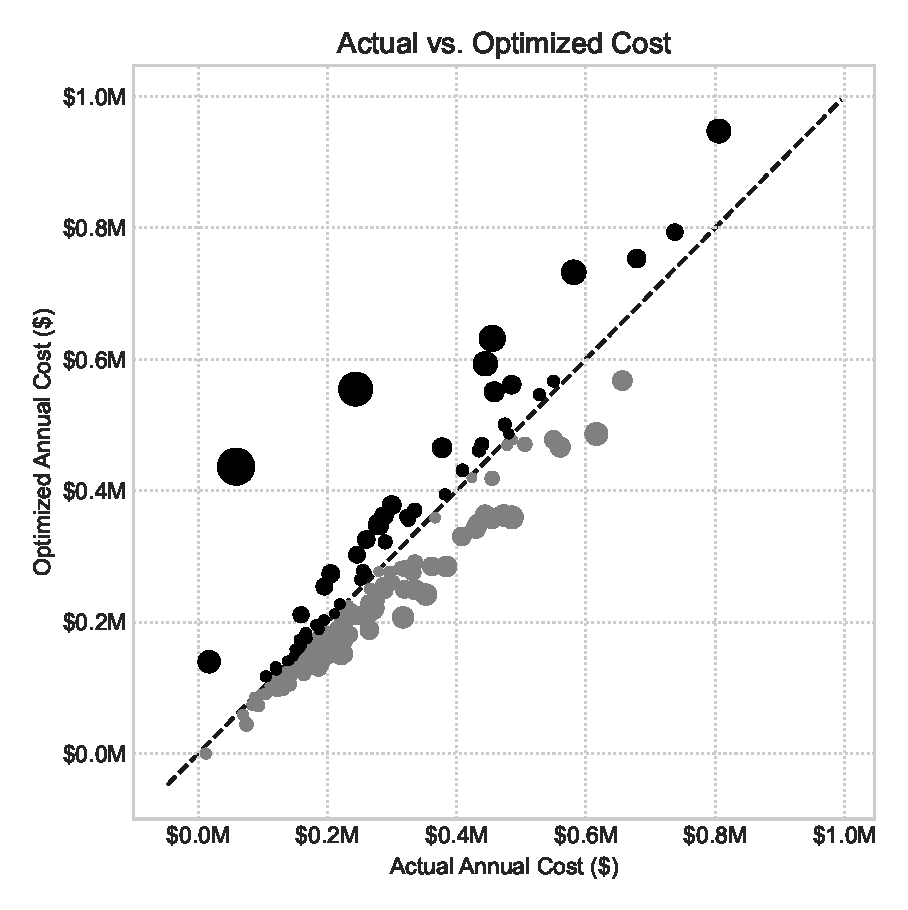
\includegraphics[width=0.8\textwidth]{fig/savings_analysis_bw.eps}
    \caption{Savings Analysis: Actual vs. Optimized Cost. Gray circles represent schools achieving savings, while black circles indicate projected losses. The size of the circle corresponds to the magnitude of the financial impact.}
    \label{fig:savings_analysis}
\end{figure*}

There is a clear correlation between school size and optimization results. The model saves the most money in schools with 500 to 1,500 students. Schools with more than 2,000 students resulted in higher costs and negative savings (see Fig. \ref{fig:savings_by_size}). Breaking down the financial data, smaller and medium-sized schools used to overproduce, which the model fixed. In contrast, larger schools may not have produced enough for their students. The model increased food allocations for these schools to ensure students are properly served.

\begin{figure}[t]
    \centering
    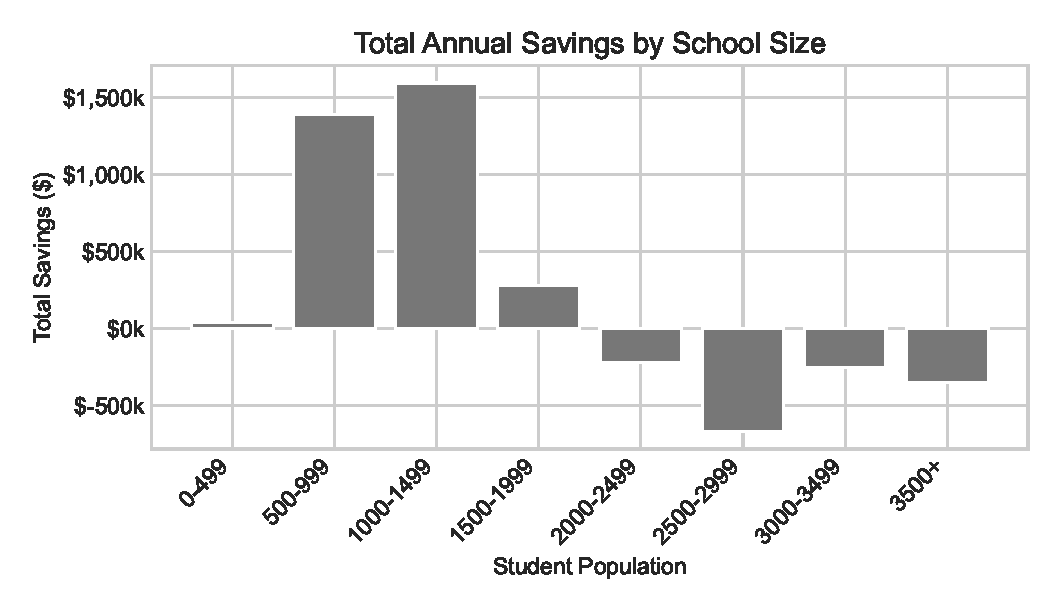
\includegraphics[width=\linewidth]{fig/savings_by_size_total_baseline.eps}
    \caption{Total Annual Savings by School Size Category. The chart shows that, by student population, the optimization model usually leads to net savings (positive values), but in some cases results in higher costs when demand constraints must be met (negative values).}
    \label{fig:savings_by_size}
\end{figure}

\subsection{Interpretation of Projected Cost Increases}
The optimization model projected a cost increase for a small group of schools, as indicated by data points above the break-even line in Fig. \ref{fig:savings_analysis}. While reverting these schools to historical production patterns may appear financially prudent, this perspective fails to account for the model's embedded constraint logic.

The optimization strictly enforces demand satisfaction constraints ($x_{s,j} \ge L_{s,j}$). This ensures production matches estimated student consumption. The historical "savings" in these schools likely result from under-production, when supply did not meet demand. This may have led to items running out or reduced service levels. The model's projected cost increase should not be seen as inefficiency, but as the \textit{true cost of service assurance}. For these schools, the model shows a gap between past budgeting and the real resources needed to fully serve students.

%*********************************************************************************************************************************************************************************************************************
\section{CHALLENGES AND LIMITATIONS}

\subsection{Challenges}

\begin{table}[t]
  \centering
  \caption{Top 10 Most Wasted Breakfast Products}
  \label{tab:breakfast_waste}
  \begin{tabular}{l S[table-format=2.1]}
    \toprule
    Product Name & {Leftover Rate (\%)} \\
    \midrule
    Fat Free Chocolate Milk(Each) & 98.8 \\
    Cereal, Cinnamon Toasters, Malt-O-Meal, IW & 60.3 \\
    Fat Free White Milk(Each) & 53.5 \\
    Cherry Flavored Dried Cranberries(Each) & 53.1 \\
    Fat Free Unflavored Shelf-Stable Milk(Each) & 52.7 \\
    Milk, Lactose Free,  Fat Free, Shelf-Stable(Each) & 51.3 \\
    Orange Flavored Dried Cranberries(Each) & 50.0 \\
    Watermelon Flavored Dried Cranberries(2 Eaches) & 48.0 \\
    Assorted Cereal(Cereal Cup) & 47.1 \\
    Patty, Chicken, Breaded, WG(2 strips) & 46.9 \\
    \bottomrule
  \end{tabular}
\end{table}

\begin{table}[t]
  \centering
  \caption{Top 10 Most Wasted Lunch Products}
  \label{tab:lunch_waste}
  \begin{tabular}{l S[table-format=2.1]}
    \toprule
    Product Name & {Leftover Rate (\%)} \\
    \midrule
    Fat Free White Milk(Each) & 60.6 \\
    Milk, Lactose Free,  Fat Free, Shelf-Stable(Each) & 50.9 \\
    1\% White Milk(Each) & 50.8 \\
    Fat Free Unflavored Shelf-Stable Milk(Each) & 48.8 \\
    Turkey,  Breast, Pre-Sliced, Oven Roasted(6 Slices) & 47.1 \\
    String Cheese(Each) & 42.8 \\
    1\% Unflavored Shelf-Stable Milk(Each) & 39.9 \\
    Assorted  4 oz Yogurt(Container) & 39.0 \\
    Mustard Packet(Packet) & 34.7 \\
    Lactose Free, White Milk(Each) & 32.9 \\
    \bottomrule
  \end{tabular}
\end{table}

An issue that other researchers observed was student acceptance of certain foods. In Mulhollem’s article \cite{mulhollem}, they observed that students, particularly elementary school students, avoided certain foods that were served to them. “Because they are the most highly wasted, understanding the extent to which fruit and vegetable offerings in school lunches are likely to be accepted by children has important implications for school meal policies and children’s health” \cite{mulhollem}. On the other side, “eggs and poultry, the researchers found, were the least-wasted food category” \cite{mulhollem}. According to our findings, milk products are the most discarded items in both \autoref{tab:breakfast_waste} and \autoref{tab:lunch_waste}. FCPS should not worry that students are avoiding their fruits and vegetables, though cranberry products are among the top 10 breakfast items wasted (\autoref{tab:breakfast_waste}). Students eating in FCPS schools are eating relatively healthy. However, with milk items frequently being wasted, this points to a problem with their waste management.

\begin{table}[t]
  \centering
  \caption{New School Menu Items for the Current School Year}
  \label{tab:new_menu_items}
  \begin{tabularx}{\linewidth}{l X}
    \toprule
    \textbf{New Product Name} & \textbf{Category} \\
    \midrule
    Cinnamon Apple Overnight Oats & Breakfast \\
    Egg \& Cheese Breakfast Quesadilla & Breakfast \\
    Egg \& Cheese Breakfast Taco & Breakfast \\
    French Toast Sticks & Breakfast \\
    Egg \& Cheese Bagel & Breakfast \\
    Turkey Sausage \& Cheese Bagel & Breakfast \\
    \midrule
    Sofritas & Lunch \\
    Peruvian Chicken Drumstick & Lunch \\
    Spanish Rice & Lunch \\
    Cheesy Turkey Pepperoni Pasta & Lunch \\
    Cheesy Pasta with Marinara Sauce & Lunch \\
    Tomato Grilled Cheese & Lunch \\
    Deep Dish Pizza & Lunch \\
    Chicken Masala Pizza & Lunch \\
    Macaroni \& Cheese & Lunch \\
    \makecell[l]{Brunch for Lunch (Cheesy Scrambled Eggs, \\ \hspace{1em}Potato Wedges, French Toast Sticks, Turkey Sausage)} & Lunch \\
    Veggie Chili & Lunch \\
    Patty Melt & Lunch \\
    Buffalo Chicken Dip & Lunch \\
    \makecell[l]{Teriyaki Chicken or Chickenless Bites Stir-Fry \\ \hspace{1em}with Fried Rice and Asian Stir-Fry Vegetables} & Lunch \\
    \bottomrule
  \end{tabularx}
\end{table}

In their study of the private school in Columbia, Missouri, Mulhollem found that changing the cafeteria menu can be difficult \cite{mulhollem}. “Addressing menu changes while staying within budget and offering children nutritious meals often is not an easy task” \cite{mulhollem}. In the 2025 school year, Fairfax County Public Schools (FCPS) introduced new menu items \cite{fcpsfood}, as shown in \autoref{tab:new_menu_items}. Since students may not be familiar with these options, there is a real risk of increased food waste if they choose not to eat them. This could worsen current waste management challenges, especially given the high production costs and large quantities involved, which may result in financial losses. Because these items are new, it will be important to conduct a follow-up study to assess their effectiveness and their impact on waste management.

Another problem brought up is the reliance on a single individual to sustain a waste management program. Huber’s article \cite{huber} describes how one teacher, Gerin Hennebaul, initiated the push for change in waste management with her students, which subsequently led to waste-management initiatives. However, if she were the only advocate for this cause and left the school, the program could collapse. In Fairfax County Public Schools, the administration is actively seeking assistance to reduce waste. This approach would require a collective effort from administrative staff and encourage passionate individuals within schools to participate. Though FCPS may be less vulnerable to this issue, it is important that the administration is committed to promoting waste management across the entire school system to ensure widespread adoption.

\subsection{Limitations}
A limitation encountered by other researchers was the narrow scope of the data. In Mulhollem’s article \cite{mulhollem}, the study observed that this school’s waste percentages align with findings from other U.S. studies. However, these results cannot be generalized to all U.S. public school cafeterias. For our study, we lacked multi-month datasets for analysis. We received food production data only for May. This snapshot did not capture the full extent of the school year’s food production and waste. Consequently, we analyzed May and inferred that the rest of the school year is comparable. Again, this inference does not represent all U.S. public school cafeterias.

We faced uncertainty about how much of the county budget goes to breakfast and lunch production. The budget documents only list unspecified 'Expenditures.' We assumed the budget includes salaries, maintenance, equipment, utilities, and compliance costs. Therefore, the amounts we present might not fit FCPS if most of a school's budget covers food production. We also assumed school budgets are allocated by size, not equally. These may not reflect the true amounts each school receives. Our analysis assumes that the Food and Nutritional Services budget primarily funds food production.


%*********************************************************************************************************************************************************************************************************************

\section{CONCLUSION}

This study tackled economic and environmental food waste issues in Fairfax County Public Schools using data analysis and an integer linear programming optimization model. The model projected an annual system-wide cost reduction of about \$1.83 million, lowering spending from \$48.94 million to \$47.11 million. This shows the system can reclaim significant economic value without lowering nutritional standards. The graphs show that the impact of optimization varies by school size. Schools with 500–1500 students had the greatest total savings, while larger schools faced a projected cost increase. This increase does not indicate inefficiency; it reveals historical under-production. The model corrects this to ensure resources fully meet student demand.

This study has some limitations related to the data used and the clarity of the budget. The analysis used production data from May to estimate yearly trends, which might not reflect seasonal changes during a full school year. Another limitation brought up was that the exact use of funds in the "Expenditures" budget category is unclear; future research will need more detailed financial data to improve cost-saving estimates. Even with these challenges, the study offers a framework for FCPS to move from its current decision-making methods to a more data-driven approach to sustainability. Therefore, FCPS should follow the recommendations generated by our model to achieve their goals to reduce their production of waste from their schools.

%*********************************************************************************************************************************************************************************************************************

\bibliographystyle{IEEEtran}
\balance
\bibliography{mybib}
\end{document}